%%%%%%%%%%%%%%%%%%%%%%%%%%%%%%%%%%%%%%%%%%%%%%%%%%%%%%%%%%%%%%%%%%%%%%%%%%%  BASIC  %%%%%%%%%%%%%%%%%%%%%%%%%%%%%%%%%%%%%%%%%%%%%%%%%%%%%%%%%%%%%%%%%%%%%%%%%%%

\section{Basic}

\subsection{Default code}
\lstinputlisting{basic/Default.cpp}

\subsection{Misc}
\lstinputlisting{basic/Misc.cpp}

\subsection{Fast read \& write}
\lstinputlisting{basic/FastRW.cpp}

\subsection{Sort cmp}
\lstinputlisting{basic/Cmp.cpp}

\subsection{Discretization}
\lstinputlisting{basic/Discretization.cpp}

\subsection{Custom unordered\_map}
\lstinputlisting{basic/CustomUnordered\_map.cpp}

\subsection{\_\_int128 read}
\lstinputlisting{basic/Int128IO.cpp}

\subsection{字典序a嚴格小於b}
\lstinputlisting{basic/LexicographicallySmaller.cpp}

\subsection{生成n位數的二進制組合}
\lstinputlisting{basic/GenBinComb.cpp}

\subsection{Radom}
\lstinputlisting{basic/Random.cpp}

%%%%%%%%%%%%%%%%%%%%%%%%%%%%%%%%%%%%%%%%%%%%%%%%%%%%%%%%%%%%%%%%%%%%%%%%%%%  Matching  %%%%%%%%%%%%%%%%%%%%%%%%%%%%%%%%%%%%%%%%%%%%%%%%%%%%%%%%%%%%%%%%%%%%%%%%%%%
\section{對拍}

\subsection{run.bat}
\lstinputlisting{matching/run.bat}

\subsection{run.sh}
\lstinputlisting{matching/run.sh}
%%%%%%%%%%%%%%%%%%%%%%%%%%%%%%%%%%%%%%%%%%%%%%%%%%%%%%%%%%%%%%%%%%%%%%%%%%%  Flow  %%%%%%%%%%%%%%%%%%%%%%%%%%%%%%%%%%%%%%%%%%%%%%%%%%%%%%%%%%%%%%%%%%%%%%%%%%%
\section{Flow \& Matching}

\subsection{Dicnic}
\lstinputlisting{flow/Dicnic.cpp}

\subsection{最大流最小花費}
\lstinputlisting{flow/ZkwFlow.cpp}

\subsection{匈牙利匹配}
\lstinputlisting{flow/Hungarian.cpp}

\subsection{KM}
\lstinputlisting{flow/KM.cpp}

%%%%%%%%%%%%%%%%%%%%%%%%%%%%%%%%%%%%%%%%%%%%%%%%%%%%%%%%%%%%%%%%%%%%%%%%%%%  Graph  %%%%%%%%%%%%%%%%%%%%%%%%%%%%%%%%%%%%%%%%%%%%%%%%%%%%%%%%%%%%%%%%%%%%%%%%%%%
\section{Graph}

\subsection{Dijkstra}
\lstinputlisting{graph/Dijkstra.cpp}

\subsection{Bellman-Ford}
\lstinputlisting{graph/Bellman-Ford.cpp}

\subsection{SPFA}
\lstinputlisting{graph/SPFA.cpp}

\subsection{Floyd-Warshall}
\lstinputlisting{graph/Floyd-Warshall.cpp}

\subsection{BCC}
\lstinputlisting{graph/BccVertex.cpp}

\subsection{SCC}
\lstinputlisting{graph/SCC.cpp}

\subsection{2SAT}
\lstinputlisting{graph/2SAT.txt}

\subsection{MaximalClique}
\lstinputlisting{graph/MaximalClique.cpp}

\subsection{MaximumClique}
\lstinputlisting{graph/MaximumClique.cpp}

\subsection{Minimum Mean Cycle}
\lstinputlisting{graph/Minimum Mean Cycle.cpp}

\subsection{Dominator Tree}
\lstinputlisting{graph/Dominator Tree.cpp}

\subsection{ManhattanMST}
\lstinputlisting{graph/ManhattanMST.cpp}

%%%%%%%%%%%%%%%%%%%%%%%%%%%%%%%%%%%%%%%%%%%%%%%%%%%%%%%%%%%%%%%%%%%%%%%%%%%  DP  %%%%%%%%%%%%%%%%%%%%%%%%%%%%%%%%%%%%%%%%%%%%%%%%%%%%%%%%%%%%%%%%%%%%%%%%%%%
\section{DP}

\subsection{數位DP}
\lstinputlisting{DP/digitDP.cpp}

\subsection{SOS DP}
\lstinputlisting{DP/SOSDP.cpp}

%%%%%%%%%%%%%%%%%%%%%%%%%%%%%%%%%%%%%%%%%%%%%%%%%%%%%%%%%%%%%%%%%%%%%%%%%%%  Math  %%%%%%%%%%%%%%%%%%%%%%%%%%%%%%%%%%%%%%%%%%%%%%%%%%%%%%%%%%%%%%%%%%%%%%%%%%%
\section{Math}

\subsection{Formulas}
\lstinputlisting{math/Formula.txt}

\subsection{llladdmul}
\lstinputlisting{math/llladdmul.cpp}

\subsection{Primes}
\lstinputlisting{math/Primes.txt}

\subsection{取樣定理}
\lstinputlisting{math/PickTheorem.cpp}

\subsection{Quick Pow}
\lstinputlisting{math/QuickPow.cpp}

\subsection{Mat quick Pow}
\lstinputlisting{math/MatPow.cpp}

\subsection{Primes Table}
\lstinputlisting{math/PrimesTable.cpp}

\subsection{Phi 函數}
\lstinputlisting{math/phi.cpp}

\subsection{Factor Table}
\lstinputlisting{math/FactorTable.cpp}

\subsection{卡塔蘭數}
\lstinputlisting{math/CatalanNumber.cpp}

\subsection{Miller Rabin}
\lstinputlisting{math/MillerRabin.cpp}

\subsection{PollarRho}
\lstinputlisting{math/PollardRho.cpp}

\subsection{PrimeFactorO(logn)}
\lstinputlisting{math/PrimeFactorO(logn).cpp}

\subsection{O(1)mul}
\lstinputlisting{math/O(1)mul.cpp}

\subsection{Josephus Problem}
\lstinputlisting{math/JosephusProblem.cpp}

\subsection{Harmonic Sum}
\lstinputlisting{math/HarmonicSum.cpp}

%%%%%%%%%%%%%%%%%%%%%%%%%%%%%%%%%%%%%%%%%%%%%%%%%%%%%%%%%%%%%%%%%%%%%%%%%%%  DataStructure  %%%%%%%%%%%%%%%%%%%%%%%%%%%%%%%%%%%%%%%%%%%%%%%%%%%%%%%%%%%%%%%%%%%%%%%%%%%
\section{Data Structure}

\subsection{BIT}
\lstinputlisting{dataStructure/BIT.cpp}

\subsection{BIT 二維}
\lstinputlisting{dataStructure/BIT2D.cpp}

\subsection{稀疏表 O(1)區間最大最小值}
\lstinputlisting{dataStructure/Sparse Table.cpp}

\subsection{Segment Tree}
\lstinputlisting{dataStructure/SegmentTree.cpp}

\subsection{動態開點線段數}
\lstinputlisting{dataStructure/dinamicSegmentTree.cpp}

\subsection{動態開點線段數 2D}
\lstinputlisting{dataStructure/dinamicSegmentTree2D.cpp}

\subsection{持久化線段樹}
\lstinputlisting{dataStructure/persistent_seg_tree.cpp}

\subsection{Time Segment Tree}
\lstinputlisting{dataStructure/TimeSegmentTree.cpp}

\subsection{Treap}
\lstinputlisting{dataStructure/Treap.cpp}

\subsection{PBDS}
\lstinputlisting{dataStructure/PBDS.cpp}

%%%%%%%%%%%%%%%%%%%%%%%%%%%%%%%%%%%%%%%%%%%%%%%%%%%%%%%%%%%%%%%%%%%%%%%%%%%  String  %%%%%%%%%%%%%%%%%%%%%%%%%%%%%%%%%%%%%%%%%%%%%%%%%%%%%%%%%%%%%%%%%%%%%%%%%%%
\section{String}

\subsection{SA}
\lstinputlisting{string/SA.cpp}

\subsection{KMP}
\lstinputlisting{string/KMP.cpp}

\subsection{Single Hash}
\lstinputlisting{string/SingleHash.cpp}

\subsection{Double Hash}
\lstinputlisting{string/DoubleHash.cpp}

\subsection{Trie}
\lstinputlisting{string/Trie.cpp}

\subsection{Z value}
\lstinputlisting{string/Zvalue.cpp}

\subsection{MinRotation}
\lstinputlisting{string/MinRotation.cpp}

\subsection{Manacher 馬拉車回文}
\lstinputlisting{string/Manacher.cpp}

\subsection{PalTree 回文樹}
\lstinputlisting{string/PalTree.cpp}

\subsection{DistinctSubsequence}
\lstinputlisting{string/DistinctSubsequence.cpp}
%%%%%%%%%%%%%%%%%%%%%%%%%%%%%%%%%%%%%%%%%%%%%%%%%%%%%%%%%%%%%%%%%%%%%%%%%%%  Tree  %%%%%%%%%%%%%%%%%%%%%%%%%%%%%%%%%%%%%%%%%%%%%%%%%%%%%%%%%%%%%%%%%%%%%%%%%%%
\section{Tree}

\subsection{LCA}
\lstinputlisting{tree/LCA.cpp}

\subsection{TreeHash}
\lstinputlisting{tree/TreeHash.cpp}

\subsection{輕重鏈剖分}
\lstinputlisting{tree/heavyLightDecomposition.cpp}
%%%%%%%%%%%%%%%%%%%%%%%%%%%%%%%%%%%%%%%%%%%%%%%%%%%%%%%%%%%%%%%%%%%%%%%%%%%  Geometry  %%%%%%%%%%%%%%%%%%%%%%%%%%%%%%%%%%%%%%%%%%%%%%%%%%%%%%%%%%%%%%%%%%%%%%%%%%%
\section{Geometry}

\subsection{2D Definition}
\lstinputlisting{geometry/2DDefinition.cpp}

\subsection{Line Definition}
\lstinputlisting{geometry/LineDefinition.cpp}

\subsection{Basic}
\lstinputlisting{geometry/Basic.cpp}

\subsection{PolygonArea}
\lstinputlisting{geometry/PolygonArea.cpp}

\subsection{IsPointInPolygon}
\lstinputlisting{geometry/IsPointInPolygon.cpp}

\subsection{ConvexHull}
\lstinputlisting{geometry/ConvexHull.cpp}

\subsection{MinkowskiSum}
\lstinputlisting{geometry/MinkowskiSum.cpp}

\subsection{Polygon Shortest Distance}
\lstinputlisting{geometry/PolygonDistance.cpp}

\subsection{ConvexHullTrick}
\lstinputlisting{geometry/ConvexHullTrick.cpp}

\subsection{Polar Sort}
\lstinputlisting{geometry/PolarSort.cpp}

\subsection{PickTheorm}
\lstinputlisting{geometry/PickTheorm.cpp}

\subsection{最近點對}
\lstinputlisting{geometry/ClosestEuclideanDistance.cpp}

\subsection{幾何中位數}
\lstinputlisting{geometry/Weiszfeld.cpp}

\subsection{矩陣掃描線}
\lstinputlisting{geometry/SweepLine.cpp}

\subsection{Circle Definition}
\lstinputlisting{geometry/CircleDefinition.cpp}

\subsection{CircleCover}
\lstinputlisting{geometry/CircleCover.cpp}

\subsection{HalfPlaneIntersection}
\lstinputlisting{geometry/HalfPlaneIntersection.cpp}

\subsection{PolygonUnion}
\lstinputlisting{geometry/PolyUnion.cpp}

\subsection{PolygonCover}
\lstinputlisting{geometry/PolyCover.cpp}

%%%%%%%%%%%%%%%%%%%%%%%%%%%%%%%%%%%%%%%%%%%%%%%%%%%%%%%%%%%%%%%%%%%%%%%%%%%  SpecialQuestion  %%%%%%%%%%%%%%%%%%%%%%%%%%%%%%%%%%%%%%%%%%%%%%%%%%%%%%%%%%%%%%%%%%%%%%%%%%%
\section{特殊題目}

\subsection{包含子字串計數}
\lstinputlisting{SpecialQuestion/ContainString.cpp}

\subsection{三維偏序}
\lstinputlisting{SpecialQuestion/Partiallyordered3D.cpp}
%%%%%%%%%%%%%%%%%%%%%%%%%%%%%%%%%%%%%%%%%%%%%%%%%%%%%%%%%%%%%%%%%%%%%%%%%%%  Python  %%%%%%%%%%%%%%%%%%%%%%%%%%%%%%%%%%%%%%%%%%%%%%%%%%%%%%%%%%%%%%%%%%%%%%%%%%%
\section{Python}

\subsection{Decimal}
\lstinputlisting{python/Decimal.py}

\subsection{Fraction}
\lstinputlisting{python/Fraction.py}

\subsection{Misc}
\lstinputlisting{python/Misc.py}
\onecolumn
\centering
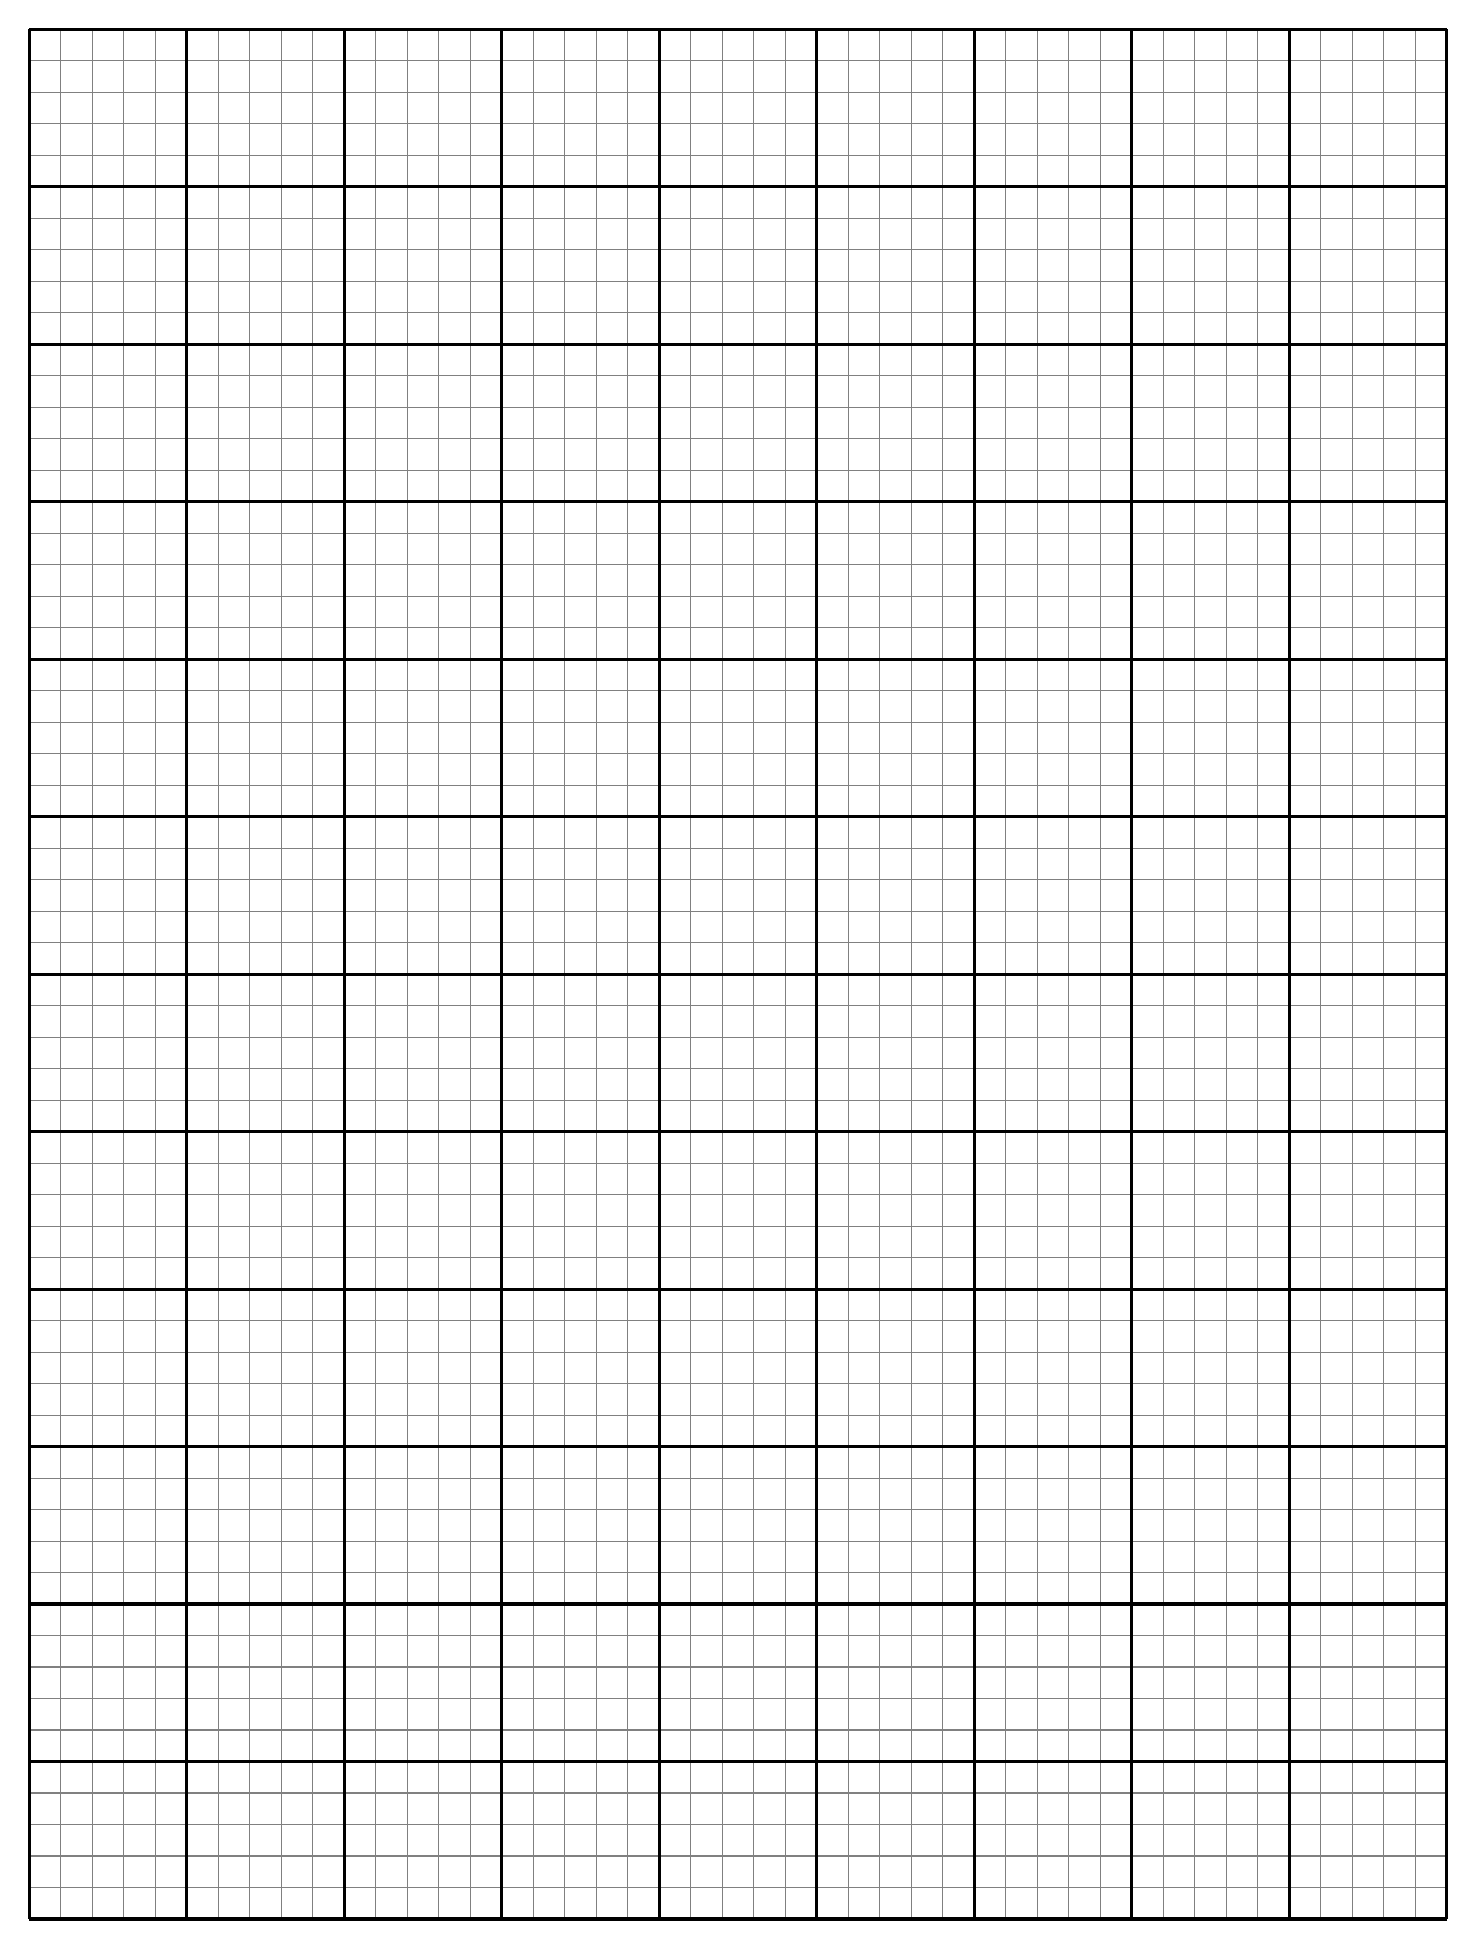
\begin{tikzpicture}[every node/.style={minimum size=1cm-\pgflinewidth, outer sep=10pt}, scale=2]
    \draw[step=0.2cm,color=gray] (0,0) grid (9,12);
    \draw[step=1cm,color=black,line width=0.4mm] (0,0) grid (9,12);
\end{tikzpicture}

\centering
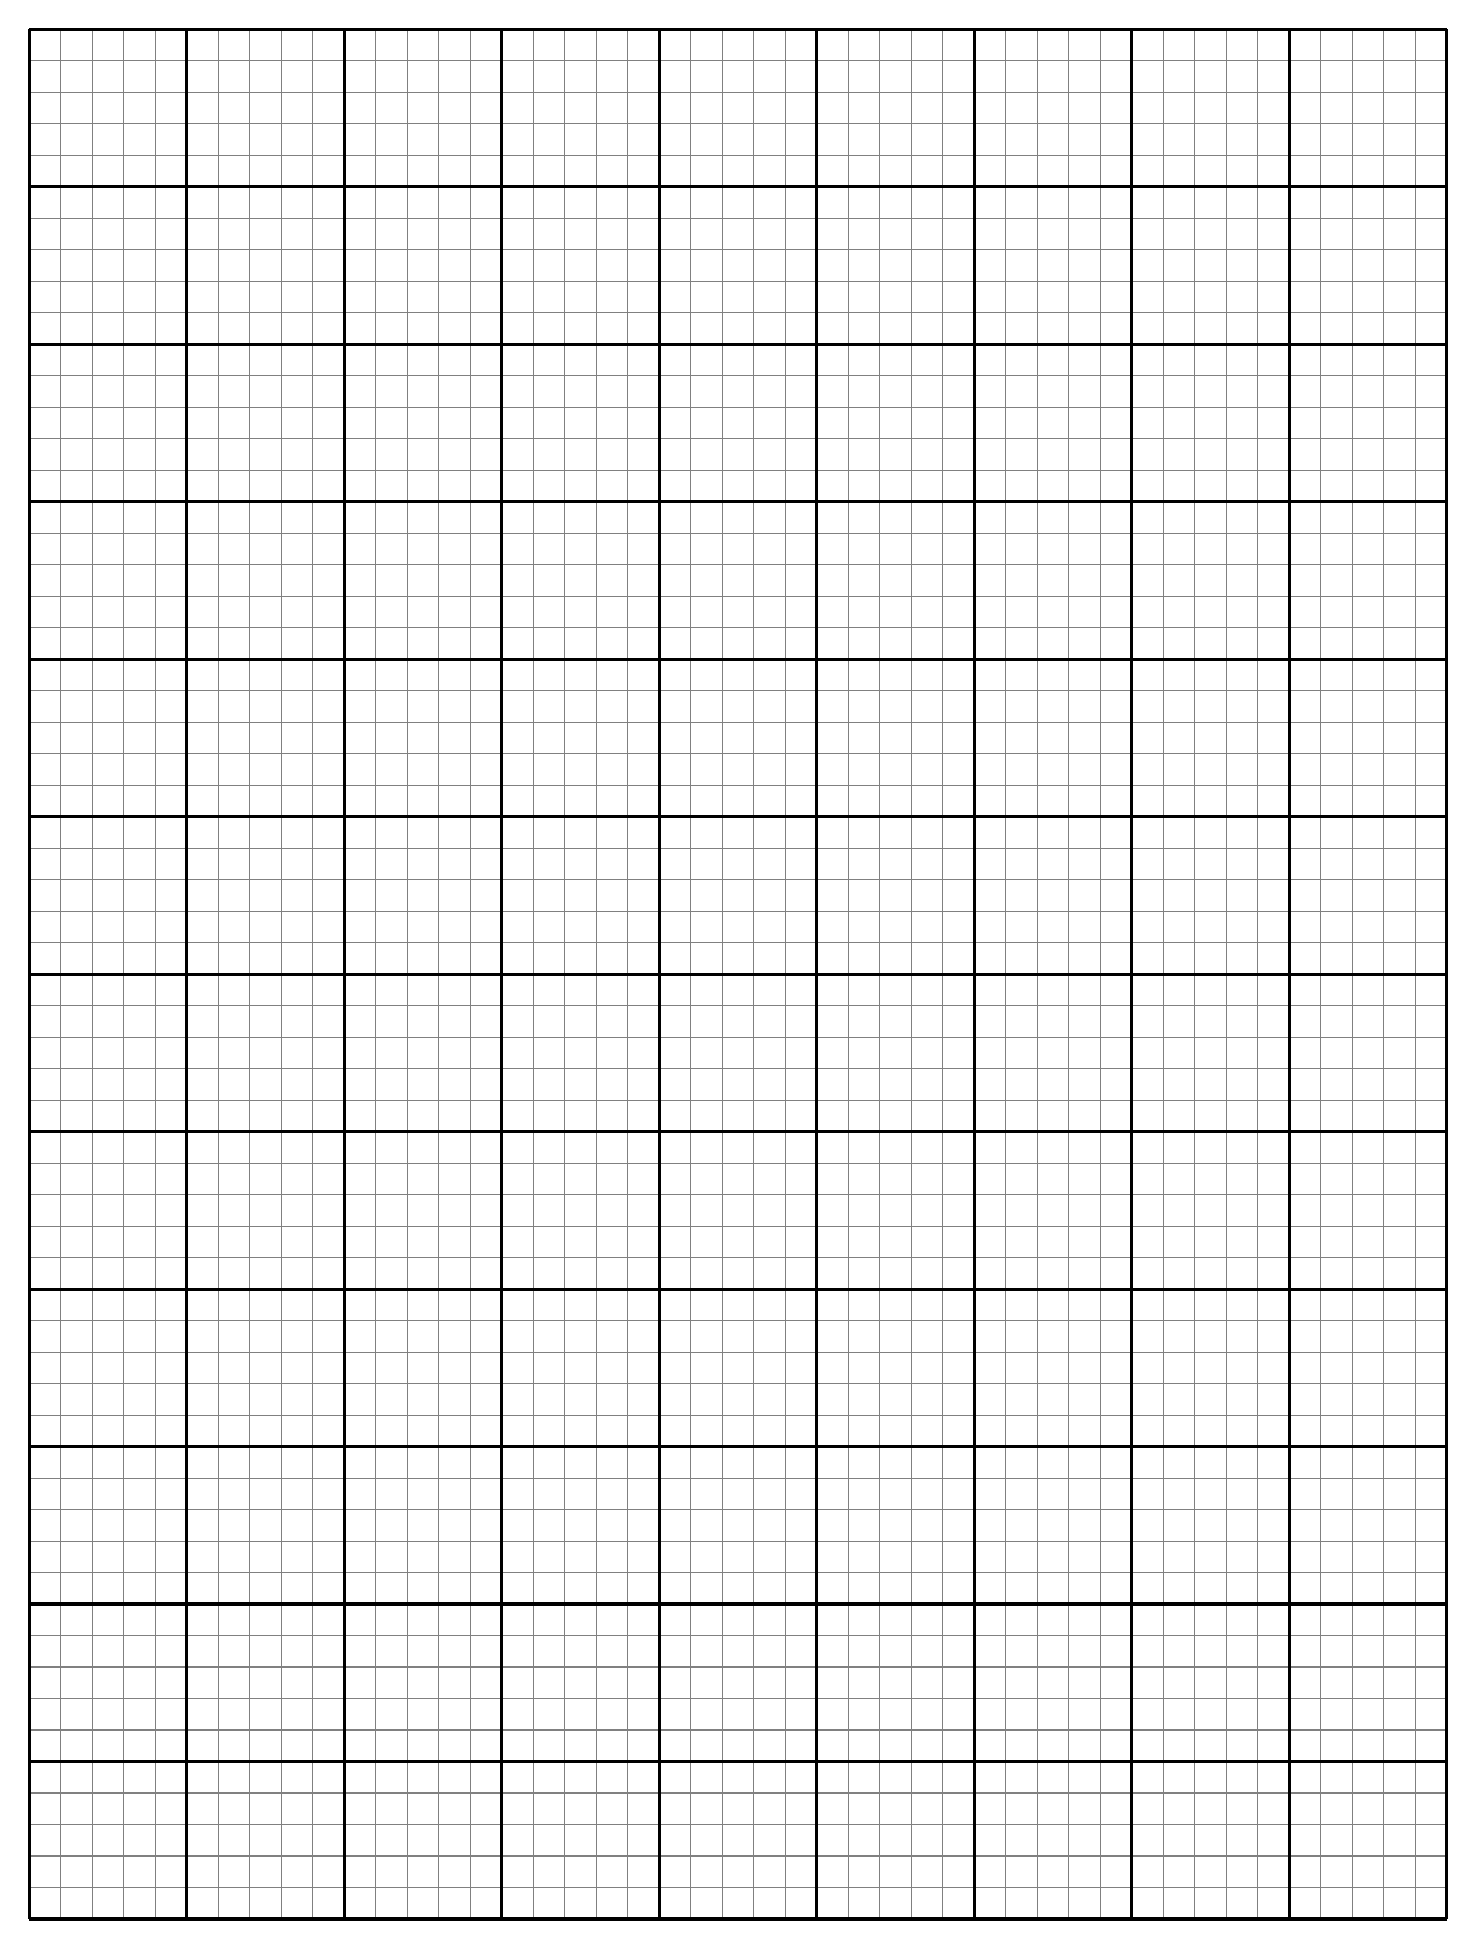
\begin{tikzpicture}[every node/.style={minimum size=1cm-\pgflinewidth, outer sep=10pt}, scale=2]
    \draw[step=0.2cm,color=gray] (0,0) grid (9,12);
    \draw[step=1cm,color=black,line width=0.4mm] (0,0) grid (9,12);
\end{tikzpicture}
